\pagestyle{myheadings}
\markboth{\nameref{sec:End}}{\nameref{sec:End}}

\chapter{Lab book 2020}

\section{Introduction}
%\markboth{Introduction}{Introduction}
%\addcontentsline{toc}{chapter}{Introduction}
Stuff about eigenvectors\index{eigenvector} and
eigenvalues\index{eigenvalue} which are being  indexed at the end of this book. 

The current classification of primary immunodeficiencies (PIDs) was compiled by the Expert Committee of the International Union of Immunological Societies
\citep{picard2018international}
in \textit{The Primary Immunodeficiency Diseases Committee Report on Inborn Errors of Immunity}.
Over approximately 50 years the list of inborn errors of immunity has grown to over 350 disorders.
I use vim snippets in my .vimrc: for producing formatting quickly including, bold face, italics, headings, and code.

\begin{lstlisting}
Computer code like this is writtin using the command. begin{lstlisting} and end{lstlisting}.
\end{lstlisting}
\marginnote{This is a margin note using the geometry package, set at 
3cm vertical offset to the line it is typeseted.}%[3cm]
Footnote example\footnote{Lorem ipsum dolor sit amet, consectetuer adipiscing elit.}.\\

\section{Sat, 8 Aug 2020 \projectA{} } 
I will add margin note after some placeholder text.
\lipsum[2-3]

\marginnote{The R script used is in "viral sequence / phylo / tree.r"}

\section{Mon, 10 Aug 2020 \projectB{}}
Working on the phylogenetic trees. 
I am producing phylogenetic trees and then splitting based on the obvious clade groups, add color, and add all labels. 
I used ggtree and ape for this work.\\
\url{ https://yulab-smu.github.io/treedata-book} \\
\url{https://4va.github.io/biodatasci/r-ggtree.html}\\
Index: phylogenetic tree, ggtree, ape.
\index{phylogenetic tree}
\index{ggtree}
\index{ape}

\section{Fri 14 Aug \projectB{} }
Here are some specific notes on a recent task.

\subsection{Processing viral data}
For \projectB{} I used ncbi-tools-bin to convert to fasta format
(note the software "Sequin" does the same job but it GUI only).
\url{https://www.huge-man-linux.net/man1/asn2fsa.html}
\index{ncbi-tools}
\begin{lstlisting}
sudo apt-get install ncbi-tools-bin
for file in rsv.*.sqn; do asn2fsa -a a -i $file -v $file.fa; done
dir: ./fa
\end{lstlisting}

Each viral genome has 11 segments that are sequenced.
With awk, I split each fasta to a new file and labelled with the read name.
i.e. segment 1 for all samples is in the file seg\_1, etc.
used \$split.sh
dir: ./seg
redo this step and split based on whole line name per fasta (remove spaces)
I used the macOS command line version of muscle to align, printing out clustal format
\begin{lstlisting}
$ for file in seg_*; do ~/Desktop/muscle3.8.31_i86darwin64 -in $file -clw -out clw.$file; done
dir: ./clw
\end{lstlisting}

I had ncbi-tools-bin installed since it runs on Debian.
I will try on my local macOS.
\url{https://ftp.ncbi.nlm.nih.gov/toolbox/ncbi_tools/}
\begin{lstlisting}
mv mac.asn2fsa ./tools/
mkdir rsv_viral_sequence_local
sync sqn dir from scitas

To extract the nucleotide from sqn.
1.export_nucleotide.sh
#!/bin/bash
# output options -v for amino, -o for nucleotide.
cd sqn
for file in rsv.*.sqn;
    do ~/tools/mac.asn2fsa -a a -i $file -o ${file%.*}.nt.fa;
done
mv ./*.nt.fa ../nt
\end{lstlisting}

Then make a simple header.
\begin{lstlisting}
$ cat 2.simplify_header.sh
#!/bin/bash
cd ./nt
for file in *.nt.fa;
    do awk -F" " '/>/{$0=$1}1' $file > ${file%.*}.nt_smp.fa ;
    done

mv ./*.nt_smp.fa ../nt_simple/

move all to post/inspire/viral_sequence/rsv_viral_seq/
\end{lstlisting}

\section{Fri, 27 Aug Lab meeting}
\subsection{Second gen P-value}
\begin{figure}[!h]
\begin{center}
  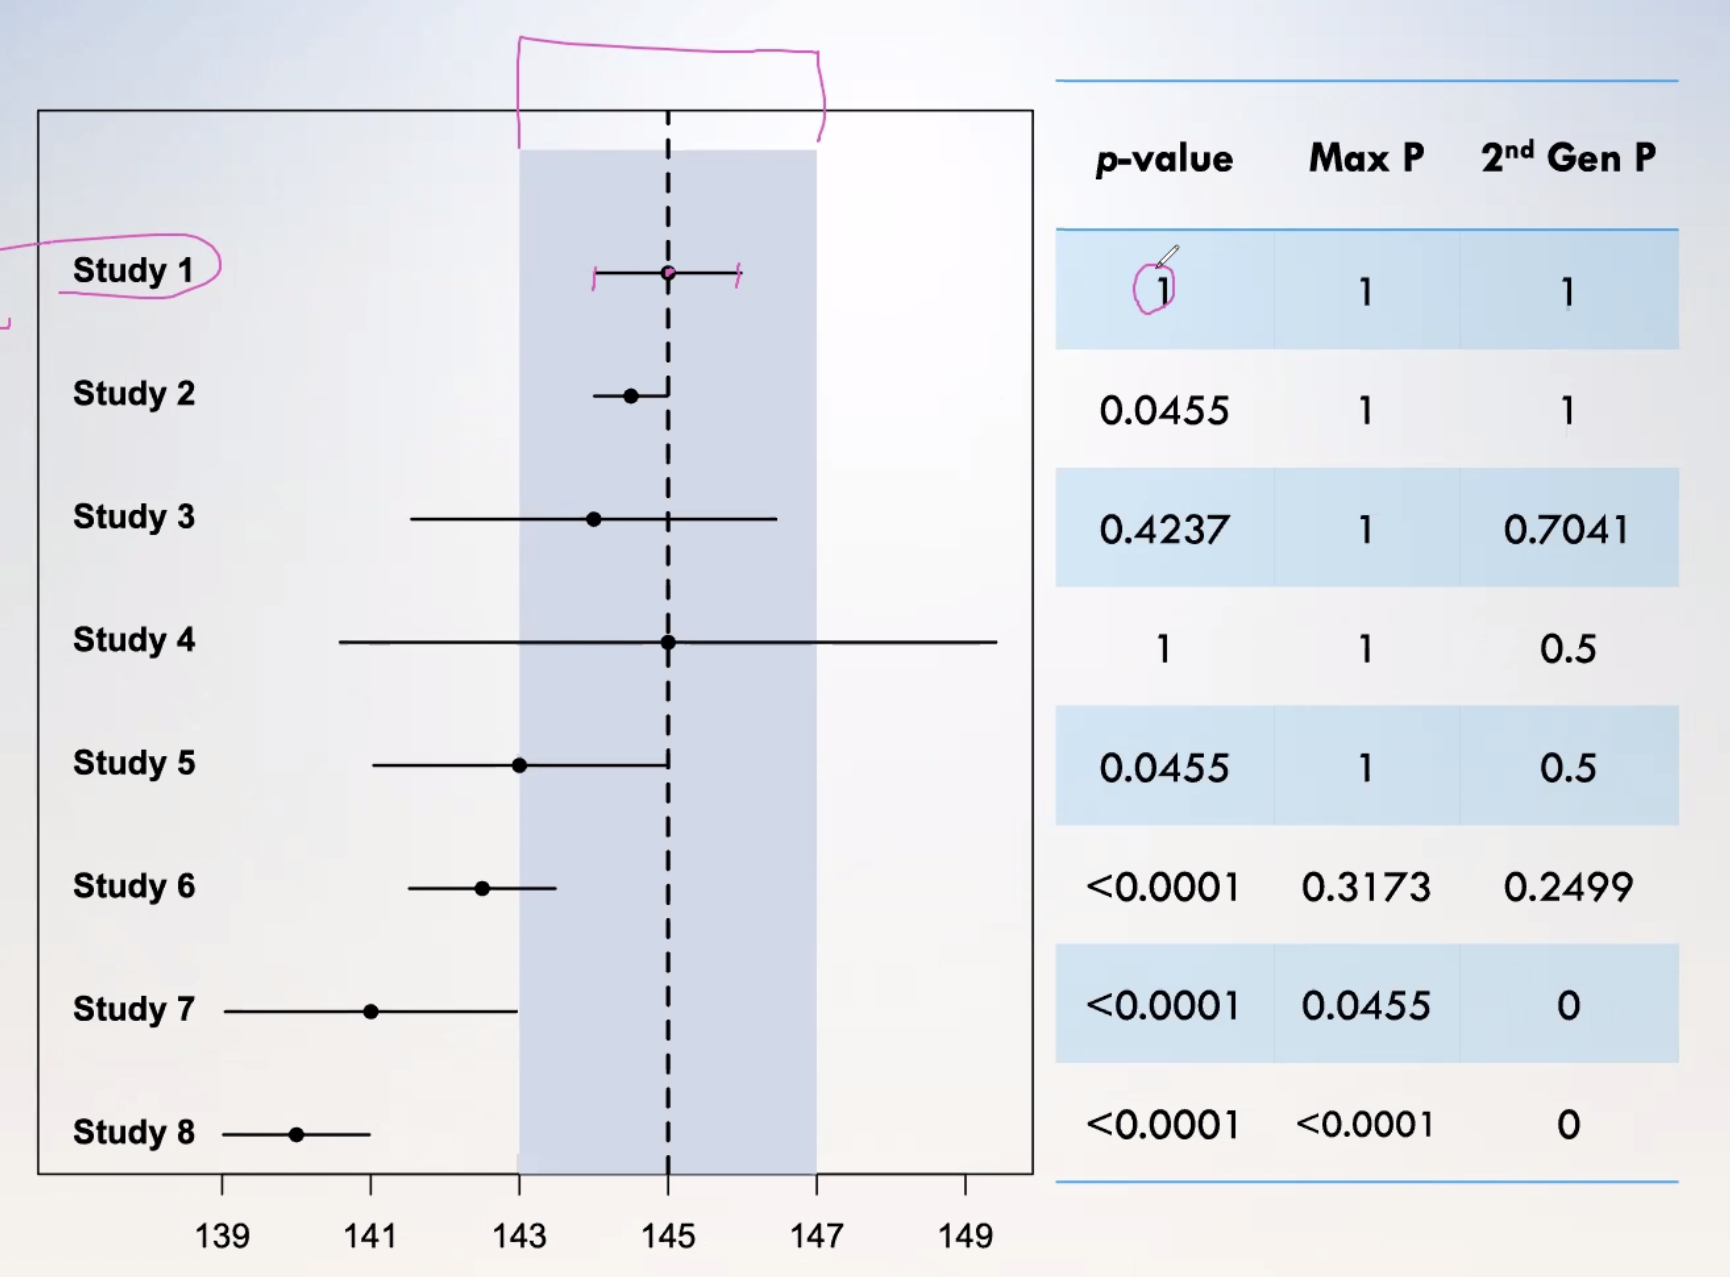
\includegraphics[scale=0.1]{misc/sgpv}
    \caption[Second gen P val]{\textbf{Second gen P val.} }
  \end{center}
\end{figure}

% Add place holder text to fill up pages and view the layout.
\lipsum[2-10]

